\section*{Motivation and Background}
\subsection*{Chapter1 : Introduction}


\subsubsection*{1.1	General problem statement }
\subsubsection*{1.2	Technical approach }
\subsubsection*{1.3 Thesis overview}
\subsubsection*{1.4 Key Contributions }
\subsubsection*{1.5 Software }
\subsubsection*{1.6 Ethics }
\subsection*{Chapter 2: Background} 
\subsubsection*{2.1 Introduction} 
\subsubsection*{2.2 Breast anatomy}
\subsubsection*{2.3 Breast imaging} 
\subsubsection*{2.4 Breast compression}

\subsubsection*{2.5 Conclusion }
\newpage
\section*{Part 2: Biomechanical breast model}
\subsection*{Chapter 3: Background and state of the art }
\subsubsection*{3.1 Introduction }
\subsubsection*{3.2 Continuous mechanics}
\subsubsection*{3.3 Finite elements theory} 
\subsubsection*{3.4 Conclusion }
\subsection*{Chapter 4: Patient specific breast biomechanical models}
\subsubsection*{4.1 Introduction }
\subsubsection*{4.2 Data acquisition} 
\subsubsection*{4.3 Finite element mesh} 
\subsubsection*{4.3 Boundary conditions} 
\subsubsection*{4.4 Tissues models} 
\subsubsection*{4.5 Stress free geometry} 
\subsubsection*{4.6 Conclusion }
\subsection*{Chapter 5: Breast mechanics modeling}
\subsubsection*{5.1 Introduction }
\subsubsection*{5.1 Boundary conditions }
\subsubsection*{5.2 Biomechanical properties of breast tissues }
\subsubsection*{5.3 Boundary conditions }
\subsubsection*{5.4 Stress-Free configuration }
\subsubsection*{5.1 Finite element mesh }
\subsubsection*{5.5 Conclusion. }
\newpage
\subsection*{Chapter6: Biomechanical breast model validation }
\subsubsection*{6.1 Introduction }
\subsubsection*{6.2 Validation process }
\subsubsection*{6.3 Breast deformation under gravity loads }
\subsubsection*{6.4 Discussions}
\subsubsection*{6.5 Conclusion  }



\section*{Part 3: Breast compression in digital mammography}
\subsection*{Chapter 7: Background}
\subsubsection*{7.1 Problem statement}
\subsubsection*{7.2 Image acquisition chain simulation} 

\subsection*{Chapter 8: Breast deformation under compression  }
\subsubsection*{8.1 Introduction }
\subsubsection*{8.1 State of the art }
\subsubsection*{8.2 Compression paddle models} 
\subsubsection*{8.3 Contact surface modeling }
\subsubsection*{8.4 Breast deformation under compression }
\subsubsection*{8.5 Discussions}
\subsubsection*{8.6 Conclusion }

\subsection*{Chapter 9: Measures of compression quality}
\subsubsection*{9.1 Introduction }
\subsubsection*{9.2 Image quality }
\subsubsection*{9.4 Breast dose }
\subsubsection*{9.5 Patient comfort}

\subsubsection*{9.6 Conclusion  }

\newpage
\subsection*{Chapter 10: Comparison of compression with different paddles geometry}
\subsubsection*{10.1 Introduction }
\subsubsection*{10.2 Gold standards }
\subsubsection*{10.3 Compression quality  }
\subsubsection*{10.4 Discussions}
\subsubsection*{10.5 Conclusion }



\section*{Part 4: Thesis review}
\subsection*{Chapter 11:  General conclusion and perspectives }
\subsubsection*{11.1 Conclusion }
\subsubsection*{11.2 Perspectives} 


%
%\section*{Abbreviations}
%\begin{itemize}
%\item IQ = image quality
%\item AGD = average glandular dose 
%\item DBT = digital breast tomosythesis
%\item Mecamat = Mecanique pour le vivant, Identification et mod\'elisation du comportement des tissus biologiques humains et animaux, Colloque National, Aussois, France, 18-22 janvier 2016
%\item ESB* = Conference of  European Society of Biomechanics, Lyon, France, 10-13 July, 2016
%\item CMBBE* =  The 14th International Symposium, Computer Methods in Biomechanics and Biomedical Engineering, Tel Aviv, Israel, 20 - 22 September, 2016
%\item SIFEM = Congr\'es de la societe francaise d'imagerie de la femme. Geneve, Suisse, 9-11 Juin 2016
%\item COSINE6 =  6th Annual International Conference in Computational Surgery. Bordeaux, France, 25-26 May,2016
%\end{itemize}
%
%* Conferences with oral presentation.
%
%\begin{center}			  
%\begin{figure}[!ht]
%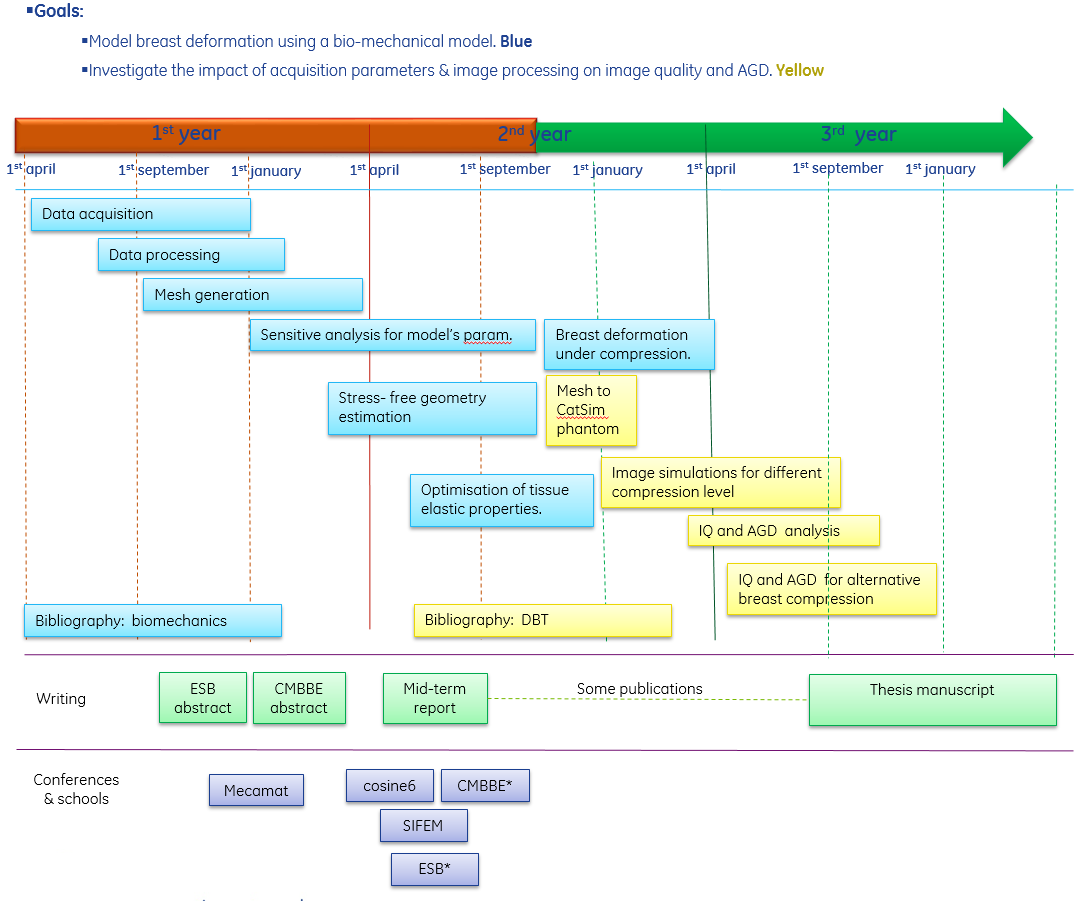
\includegraphics[width=\textwidth,height=\textheight,keepaspectratio]{figures/researchPlan.png} 
%\label{researchPlan}
%\end{figure}
%\end{center}
%
%\chapter{Followed training}
%
%\begin{center}			  
%\begin{figure}[!ht]
%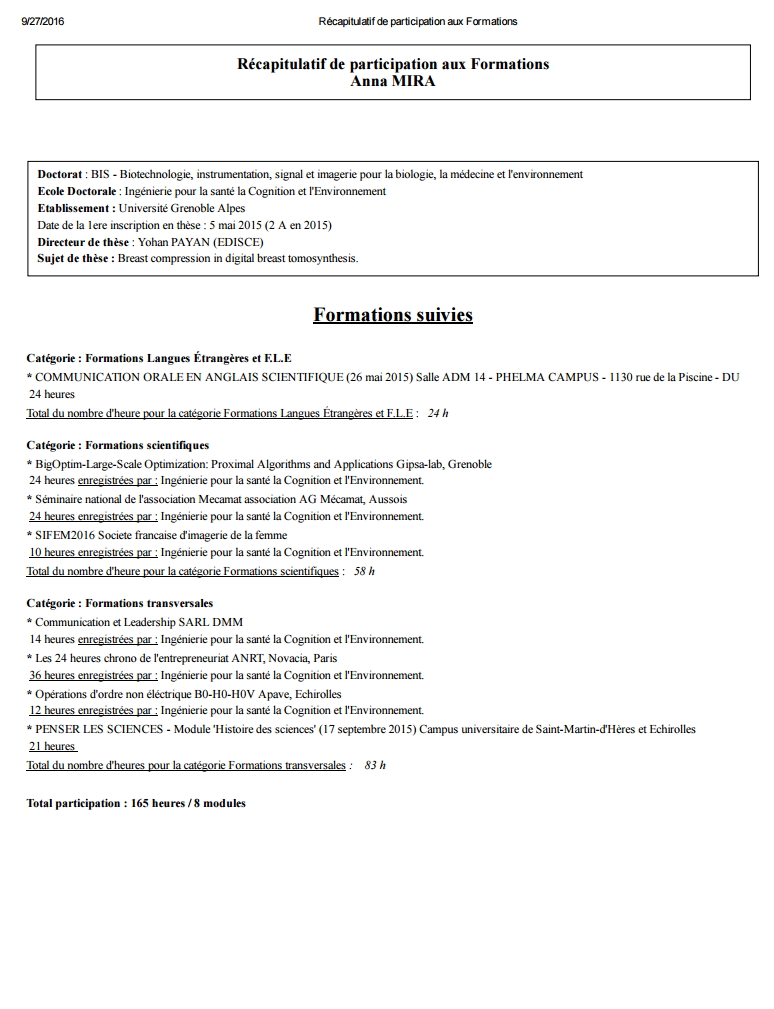
\includegraphics[scale=1]{figures/formation.PNG} 
%\label{formation}
%\end{figure}
%\end{center}